\section{Inequalities and means}
\secbegin{secInequalitiesMeans}

We first encountered the real numbers in \Cref{chGettingStarted}, when the real numbers were introduced using a vague (but intuitive) notion of an \textit{infinite number line} (\Cref{defRealsInformal}):

\begin{center}
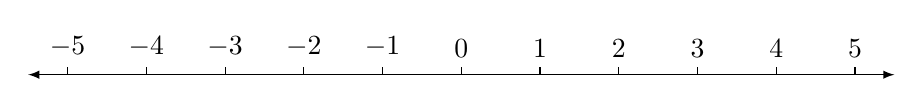
\begin{tikzpicture}
\draw[latex-latex] (-5.5, 0) -- (5.5, 0) ; 
\foreach \x in {-5,-4,-3,-2,-1,0,1,2,3,4,5} \draw (\x, 0) -- (\x, 0.1) node[above] {$\x$} ;
\end{tikzpicture}
\end{center}

This section will scrutinise the set of real numbers in its capacity as a \textit{complete ordered field}. Decomposing what this means:
\begin{itemize} 
\item A \textit{field} is a set with a notion of `zero' and `one', in which it makes sense to talk about addition, subtraction, multiplication, and division by everything except zero. Examples are $\mathbb{Q}$, $\mathbb{R}$, and $\mathbb{Z}/p\mathbb{Z}$ when $p$ is a prime number (but not when $p$ is composite). However, $\mathbb{Z}$ is not a field, since we can't freely divide by nonzero elements---for example, $1 \in \mathbb{Z}$ and $2 \in \mathbb{Z}$, but no integer $n$ satisfies $2n=1$.
\item An \textit{ordered field} is a field which is equipped with a well-behaved notion of order. Both $\mathbb{Q}$ and $\mathbb{R}$ are ordered fields, but $\mathbb{Z}/p\mathbb{Z}$ is not. We'll see why soon.
\item A \textit{complete ordered field} is an ordered field in which every set with an upper bound has a \textit{least} upper bound. As we will see, $\mathbb{Q}$ is not a complete ordered field, but $\mathbb{R}$ is.
\end{itemize}

This is made (extremely) precise in \Cref{secConstructions}.

\subsection*{Magnitude and scalar product}

In this part of the section, we home in on sets of the form $\mathbb{R}^n$, for $n \in \mathbb{N}$. Elements of $\mathbb{R}^n$ are sequences of the form $(x_1,x_2,\dots,x_n)$, where each $x_i \in \mathbb{R}$. With our interpretation of the reals $\mathbb{R}$ as a \textit{line}, we can interpret a sequence $(x_1,x_2,\dots,x_n)$ as a point in \textit{$n$-dimensional space}:
\begin{itemize}
\item $0$-dimensional space is a single point. The set $\mathbb{R}^0$ has one element, namely the empty sequence $()$, so this makes sense.
\item $1$-dimensional space is a line. This matches our intuition that $\mathbb{R}=\mathbb{R}^1$ forms a line.
\item $2$-dimensional space is a \textit{plane}. The elements of $\mathbb{R}^2$ are pairs $(x,y)$, where $x$ and $y$ are both real numbers. We can interpret the pair $(x,y)$ as \textit{coordinates} for a point which is situated $x$ units to the right of $(0,0)$ and $y$ units above $(0,0)$ (where negative values of $x$ or $y$ reverse this direction)---see \Cref{figPointsInR2}.
\end{itemize}

\begin{figure}[ht]
\centering
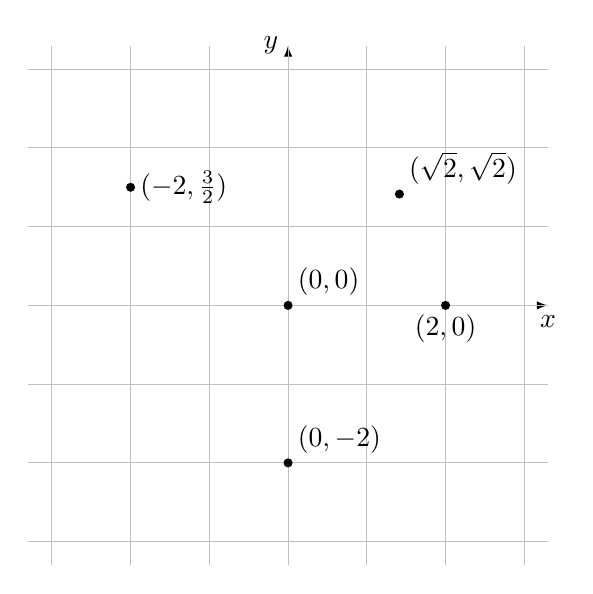
\begin{tikzpicture}
\draw[-latex] (-3.3, 0) -- (3.3, 0) node[below] {$x$} ;
\draw[-latex] (0, -3.3) -- (0, 3.3) node[left] {$y$} ;
\foreach \x in {-3,-2,-1,0,1,2,3} \draw[lightgray] (\x, -3.3) -- (\x, 3.3) ;
\foreach \y in {-3,-2,-1,0,1,2,3} \draw[lightgray] (-3.3, \y) -- (3.3, \y) ;
\draw[fill] (0,0) circle[radius=0.05] node[above right] {$(0,0)$} ;
\draw[fill] ({sqrt(2)},{sqrt(2)}) circle[radius=0.05] node[above right] {$(\sqrt{2},\sqrt{2})$} ;
\draw[fill] (0,-2) circle[radius=0.05] node[above right] {$(0,-2)$} ;
\draw[fill] (2,0) circle[radius=0.05] node[below] {$(2,0)$} ;
\draw[fill] (-2,1.5) circle[radius=0.05] node[right] {$(-2, \frac{3}{2})$} ;
\end{tikzpicture}
\caption{Some points in $\mathbb{R}^2$}
\label{figPointsInR2}
\end{figure}

With this intuition in mind, we set up the following notation.

\begin{notation}
\label{ntnVectorsInRn}
\index{origin}
\index{component}
Let $n \in \mathbb{N}$. Elements of $\mathbb{R}^n$ will be denoted $\vec x, \vec y, \vec z, \dots$\nindex{xvec}{$\vec x$}{vector} \inlatex{vec}\lindexmmc{vec}{$\vec a, \vec b, \dots$} and called ($n$-\textbf{dimensional}) \textbf{vectors}. Given a vector $\vec x \in \mathbb{R}^n$, we write $x_i$ for the $i^{\text{th}}$ \textbf{component} of $\vec x$, so that
\[ \vec x = (x_1,x_2,\dots,x_n) \]
The element $(0,0,\dots,0) \in \mathbb{R}^n$ is called the \textbf{origin} or \textbf{zero vector} of $\mathbb{R}^n$, and is denoted by $\vec 0$.

Moreover, if $\vec x, \vec y \in \mathbb{R}^n$ and $a \in \mathbb{R}$ we write
\[ \vec x + \vec y = (x_1+y_1,x_2+y_2,\dots,x_n+y_n) \quad \text{and} \quad a \vec x = (ax_1,ax_2,\dots,ax_n) \]
\end{notation}

\begin{example}
For all $\vec x \in \mathbb{R}^n$, we have
\[ \vec x + \vec 0 = \vec x \quad \text{and} \quad 1 \vec x = \vec x \]
\end{example}

\begin{definition}
\label{defMagnitude}
\index{magnitude}
\index{distance}
Let $\vec x \in \mathbb{R}^n$. The \textbf{magnitude} of $\vec x$ is the real number $\lVert \vec x \rVert$\nindex{xmag}{$\lVert \vec x \rVert$}{magnitude} \inlatex{lVert\ \textbackslash{}vec\ x\ \textbackslash{}rVert}\lindexmmc{lVert\dots{}\textbackslash{}rVert}{$\lVert \dots{} \rVert$} defined by
\[ \lVert \vec x \rVert = \sqrt{\sum_{i=1}^n x_i^2} = \sqrt{x_1^2+x_2^2+\cdots+x_n^2} \]
Given vectors $\vec x, \vec y \in \mathbb{R}^n$, the \textbf{distance} from $\vec x$ to $\vec y$ is defined to be $\lVert \vec y - \vec x \rVert$. Thus the magnitude of a vector can be thought of as the distance from that vector to the origin.
\end{definition}

\begin{example}
\label{exMagnitudeInR2}
In $\mathbb{R}^2$, \Cref{defMagnitude} says that
\[ \lVert (x,y) \rVert = \sqrt{x^2+y^2} \]
This matches the intuition obtained from the Pythagorean theorem on the sides of right-hand triangles. For example, consider the triangle with vertices $(0,0)$, $(4,0)$ and $(4,3)$:
\begin{center}
\begin{tikzpicture}
\draw (0,0) node [below left] {$(0,0)$}
   -- (4,0) node [below right] {$(4,0)$}
   -- (4,3) node [above right] {$(4,3)$}
   -- (0,0) ;
\end{tikzpicture}
\end{center}
The hypotenuse of the triangle has magnitude
\[ \lVert (4,3) \rVert = \sqrt{4^2+3^2} = \sqrt{25} = 5 \]
\end{example}

\begin{exercise}
\label{exDistanceIsSymmetric}
Let $\vec x, \vec y \in \mathbb{R}^n$. Prove that $\lVert \vec x - \vec y \rVert = \lVert \vec y - \vec x \rVert$. That is, the distance from $\vec x$ to $\vec y$ is equal to the distance from $\vec y$ to $\vec x$.
\end{exercise}

\begin{exercise}
Prove that if $x \in \mathbb{R}$ then the magnitude $\lVert (x) \rVert$ is equal to the absolute value $|x|$.
\end{exercise}

\begin{exercise}
\label{exVectorZeroIffMagnitudeZero}
Let $\vec x \in \mathbb{R}^n$. Prove that $\lVert \vec x \rVert = 0$ if and only if $\vec x = \vec 0$.
\end{exercise}

\subsection*{The triangle inequality and the Cauchy--Schwarz inequality}

The first, and simplest, inequality that we investigate is the (one-dimensional version of the) \textit{triangle inequality} (\Cref{thmTriangleInequality1D}). It is so named because of a generalisation to higher dimensions (\Cref{thmTriangleInequality}), which can be interpreted geometrically as saying that the sum of two side lengths of a triangle is greater than or equal to the third side length.

The triangle inequality is used very frequently in mathematical proofs---you will encounter it repeatedly in this chapter---yet its proof is surprisingly simple.

Before we can prove the triangle inequality, we need the following fact about square roots of real numbers.

\begin{lemma}
\label{lemSquareRootIsOrderPreserving}
Let $x,y \in \mathbb{R}$. If $0 \le x \le y$, then $\sqrt{x} \le \sqrt{y}$.
\end{lemma}
\begin{cproof}
Suppose $0 \le x \le y$. Note that, by definition of the square root symbol, we have $\sqrt{x} \ge 0$ and $\sqrt{y} \ge 0$.

Suppose $\sqrt{x} > \sqrt{y}$. By two applications of \Cref{thmPropertiesOfOrderedFields}(d), we have
\[ y = \sqrt{y} \cdot \sqrt{y} < \sqrt{x} \cdot \sqrt{y} < \sqrt{x} \cdot \sqrt{x} = x \]
so that $y<x$. But this contradicts the assumption that $x \le y$. Hence $\sqrt{x} \le \sqrt{y}$, as required.
\end{cproof}

\begin{theorem}[Triangle inequality in one dimension]
\label{thmTriangleInequality1D}
\index{triangle inequality!in one dimension}
\index{inequality!triangle (one-dimensional)}
Let $x,y \in \mathbb{R}$. Then $|x+y| \le |x|+|y|$. Moreover, $|x+y|=|x|+|y|$ if and only if $x$ and $y$ have the same sign.
\end{theorem}
\begin{cproof}
Note first that $xy \le |xy|$; indeed, $xy$ and $|xy|$ are equal if $xy$ is non-negative, and otherwise we have $xy < 0 < |xy|$. Also $x^2=|x|^2$ and $y^2=|y|^2$. Hence
\[ (x+y)^2 = x^2+2xy+y^2 \le |x|^2+2|xy|+|y|^2 = (|x|+|y|)^2 \]
Taking (nonnegative) square roots yields
\[ |x+y| \le ||x|+|y|| \]
by \Cref{lemSquareRootIsOrderPreserving}. But $|x|+|y| \ge 0$, so $||x|+|y||=|x|+|y|$. This completes the first part of the proof.

Equality holds in the above if and only if $xy=|xy|$, which occurs if and only if $xy \ge 0$. But this is true if and only if $x$ and $y$ are both non-negative or both non-positive---that is, they have the same sign.
\end{cproof}

\begin{example}
Let $x,y \in \mathbb{R}$. We prove that
\[ \frac{|x+y|}{1+|x+y|} \le \frac{|x|}{1+|x|} + \frac{|y|}{1+|y|} \]
First note that, if $0 \le s \le t$, then
\[ \frac{s}{1+s} \le \frac{t}{1+t} \]
To see this, note that
\begin{align*}
s \le t &\Rightarrow 1+s \le 1+t && \text{rearranging} \\
&\Rightarrow \frac{1}{1+t} \le \frac{1}{1+s} && \text{since $1+s,1+t > 0$} \\
&\Rightarrow 1-\frac{1}{1+s} \le 1-\frac{1}{1+t} && \text{rearranging} \\
&\Rightarrow \frac{s}{1+s} \le \frac{t}{1+t} && \text{rearranging}
\end{align*}
Now letting $s=|x+y|$ and $t=|x|+|y|$, we have $s \le t$ by the triangle inequality, and hence
\[ \frac{|x+y|}{1+|x+y|} \le \frac{|x|}{{1+|x|+|y|}} + \frac{|y|}{1+|x|+|y|} \le \frac{|x|}{1+|x|} + \frac{|y|}{1+|y|} \]
as required.
\end{example}

\begin{exercise}
Let $n \in \mathbb{N}$ and let $x_i \in \mathbb{R}$ for each $i \in [n]$. Prove that
\[ \left| \sum_{i=1}^n x_i \right| \le \sum_{i=1}^n |x_i| \]
with equality if and only if the numbers $x_i$ are either all non-positive or all non-negative.
\end{exercise}

\begin{exercise}
Let $x,y \in \mathbb{R}$. Prove that
\[ ||x|-|y|| \le |x-y| \]
\end{exercise}

We will generalise the triangle inequality to arbitrary dimensions in \Cref{thmTriangleInequality}. Our proof will go via the \textit{Cauchy--Schwarz inequality} (\Cref{thmCauchySchwarzInequality}). To motivate the Cauchy--Schwarz inequality, we introduce another geometric notion called the \textit{scalar product} of two vectors.

\begin{definition}
\label{defScalarProduct}
\index{scalar product}
\index{dot product}
Let $\vec x,\vec y \in \mathbb{R}^n$. The \textbf{scalar product} (or \textbf{dot product}) of $\vec x$ with $\vec y$ is the real number $\vec x \cdot \vec y$\nindex{xdoty}{$\vec x \cdot \vec y$}{scalar product} \inlatex{cdot}\lindexmmc{cdot}{$\cdot$} defined by
\[ \vec x \cdot \vec y = \sum_{i=1}^n x_iy_i = x_1y_1+x_2y_2+\cdots+x_ny_n \]
\end{definition}

\begin{example}
\label{exVectorDotItself}
Let $\vec x \in \mathbb{R}^n$. Then $\vec x \cdot \vec x = \lVert \vec x \rVert^2$. Indeed
\[ \vec x \cdot \vec x = \sum_{i=1}^n x_i^2 = \lVert \vec x \rVert^2 \]
\end{example}

\begin{exercise}
\label{exScalarProductIsBilinear}
Let $\vec x, \vec y, \vec z, \vec w \in \mathbb{R}^n$ and let $a,b,c,d \in \mathbb{R}$. Prove that
\[ (a \vec x + b \vec y) \cdot (c \vec z + d \vec w) = ac (\vec x \cdot \vec z) + ad (\vec x \cdot \vec w) + bc( \vec y \cdot \vec z) + bd (\vec y \cdot \vec w) \]
\end{exercise}

Intuitively, the scalar product of two vectors $\vec x$ and $\vec y$ measures the extent to which $\vec x$ and $\vec y$ fail to be \textit{orthogonal}. In fact, if $\theta$ is the acute angle formed between the lines $\ell_1$ and $\ell_2$, where $\ell_1$ passes through $\vec 0$ and $\vec x$ and $\ell_2$ passes through $\vec 0$ and $\vec y$, then a formula for the scalar product of $\vec x$ and $\vec y$ is given by
\[ \vec x \cdot \vec y = \lVert \vec x \rVert \lVert \vec y \rVert \cos \theta \]

\begin{center}
\begin{tikzpicture}[scale=1.5]
\draw [->] (0,0) node [left] {$\vec 0$}
        -- (4,2) node [above right] {$\vec x$} ;
\draw [->] (0,0)
        -- (5,0) node [right] {$\vec y$} ;
\draw [dashed] (4,2) -- (4,0) ;
\draw (3.7,0) -- (3.7,0.3) -- (4,0.3) ;
\draw [<->] (0,-0.3) -- (4,-0.3) ;
\node [below] at (2,-0.3) {$\lVert x \rVert \cos \theta$} ;
\draw [->, domain=0:atan(0.5)] plot ({0.7*cos(\x)},{0.7*sin(\x)}) ;
\node at ({0.85*cos(atan(0.25))}, {0.85*sin(atan(0.25))}) {$\theta$} ;
\end{tikzpicture}
\end{center}

Evidently, $\vec x$ and $\vec y$ are orthogonal if and only if $\cos \theta = 0$, in which case $\vec x \cdot \vec y = 0$ as well. We cannot prove this yet, though, as we have not yet defined trigonometric functions or explored their properties, but hopefully this provides some useful intuition.

The Cauchy--Schwarz inequality provides a useful comparison of the size of a scalar product of two vectors with the magnitudes of the vectors.

\begin{theorem}[Cauchy--Schwarz inequality]
\label{thmCauchySchwarzInequality}
\index{Cauchy--Schwarz inequality}
\index{inequality!Cauchy--Schwarz}
Let $n \in \mathbb{N}$ and let $x_i,y_i \in \mathbb{R}$ for each $i \in [n]$. Then
\[ |\vec x \cdot \vec y| \le \lVert \vec x \rVert \lVert \vec y \rVert \]
with equality if and only if $a\vec x = b\vec y$ for some $a,b \in \mathbb{R}$ which are not both zero.
\end{theorem}
\begin{cproof}
If $\vec y = \vec 0$, then this is trivial: both sides of the equation are equal to zero! So assume that $\vec y \ne \vec 0$. In particular, by \Cref{exVectorZeroIffMagnitudeZero}, we have $\lVert \vec y \rVert > 0$.

Define $k = \dfrac{\vec x \cdot \vec y}{\lVert \vec y \rVert^2}$. Then
\begin{align*}
0 &\le \lVert \vec x - k \vec y \rVert^2 && \text{since squares are nonnegative} \\
&= (\vec x - k \vec y) \cdot (\vec x - k \vec y) && \text{by \Cref{exVectorDotItself}} \\
&= (\vec x \cdot \vec x) - 2k (\vec x \cdot \vec y) + k^2 (\vec y \cdot \vec y) && \text{by \Cref{exScalarProductIsBilinear}} \\
&= \lVert \vec x \rVert^2 - \frac{(\vec x \cdot \vec y)^2}{\lVert y \rVert^2} && \text{by definition of $k$}
\end{align*}
Multiplying through by $\lVert \vec y \rVert^2$, which is non-negative and therefore doesn't change the sign of the inequality, yields
\[ 0 \le \lVert \vec x \rVert^2 \lVert \vec y \rVert^2 - (\vec x \cdot \vec y)^2 \]
which is equivalent to what was to be proved.

Evidently, equality holds if and only if $\lVert \vec x - k \vec y \rVert = 0$, which by \Cref{exVectorZeroIffMagnitudeZero} occurs if and only if $\vec x - k \vec y = 0$. Now:
\begin{itemize}
\item If $\vec x - k\vec y = 0$, then we have
\begin{align*}
&\vec x - k \vec y = 0 && \\
&\Leftrightarrow \vec x - \frac{\vec x \cdot \vec y}{\lVert \vec y \rVert^2} \vec y = 0 && \text{by definition of $k$} \\
&\Leftrightarrow \lVert \vec y \rVert^2 \vec x = (\vec x \cdot \vec y) \vec y && \text{rearranging}
\end{align*}
%% BEGIN EXTRACT (xtrProvingExistsExampleTwo) %%
If $\vec y \ne \vec 0$ then let $a=\lVert \vec y \rVert^2$ and $b=\vec x \cdot \vec y$; otherwise, let $a=0$ and $b=1$. In both cases, we have $a \vec x = b \vec y$ and $a,b$ are not both zero.
%% END EXTRACT %%

If $a \vec x = b \vec y$ for some $a,b \in \mathbb{R}$ not both zero, then either:
\begin{itemize}
\item $a=0$ and $b \ne 0$, in which case $\vec y = 0$ and we have equality in the Cauchy--Schwarz inequality; or
\item $a \ne 0$, in which case $\vec y = \frac{b}{a} \vec x$. Write $c=\frac{b}{a}$. Then
\begin{align*}
|\vec x \cdot \vec y| &= | \vec x \cdot (c \vec x) | && \\
&= |c(\vec x \cdot \vec x)| && \text{by \Cref{exScalarProductIsBilinear}} \\
&= |c| \lVert \vec x \rVert^2 && \text{by \Cref{exVectorDotItself}} \\
&= \lVert \vec x \rVert \lVert c \vec x \rVert && \text{rearranging} \\
&= \lVert \vec x \rVert \lVert \vec y \rVert &&
\end{align*}
\end{itemize}
In either case, we have equality in the Cauchy--Schwarz inequality.
\end{itemize}

So equality holds if and only if $a \vec x = b \vec y$ for some $a,b \in \mathbb{R}$ not both zero.
\end{cproof}

\begin{example}
Let $a,b,c \in \mathbb{R}$. We'll prove that
\[ ab+bc+ca \le a^2+b^2+c^2 \]
and examine when equality holds.

Letting $\vec x = (a,b,c)$ and $\vec y = (b,c,a)$ yields
\[ \vec x \cdot \vec y = ab+bc+ca \]
and
\[ \lVert \vec x \rVert = \sqrt{a^2+b^2+c^2} = \sqrt{b^2+c^2+a^2} = \lVert \vec y \rVert \]
Hence $\lVert \vec x \rVert \lVert \vec y \rVert = a^2+b^2+c^2$. By the Cauchy--Schwarz inequality, it follows that
\[ \vec x \cdot \vec y = ab+bc+ca \le a^2+b^2+c^2 = \lVert \vec x \rVert \lVert \vec y \rVert \]
as required. Equality holds if and only if $k(a,b,c) = \ell(b,c,a)$ for some $k,\ell \in \mathbb{R}$ not both zero. We may assume $k \ne 0$---otherwise, swap the vectors $\vec x$ and $\vec y$ in what follows. Then, letting $t=\frac{\ell}{k}$, we have
\begin{align*}
&k(a,b,c) = \ell(b,c,a) && \\
&\Leftrightarrow (a,b,c) = (tb,tc,ta) && \text{by definition of $t$} \\
&\Leftrightarrow (a,b,c) = (t^2c,t^2a,t^2b) && \text{substituting $a=tb$ etc.} \\
&\Leftrightarrow (a,b,c) = (t^3a,t^3b,t^3c) && \text{substituting $a=tb$ etc.\ again} \\
&\Leftrightarrow \vec x = t^3 \vec x
\end{align*}
This occurs if and only if either $(a,b,c)=(0,0,0)$, or $t=1$, in which case
\[ (a,b,c) = (tb,tc,ta) = (b,c,a) \]
So equality holds if and only if $a=b=c$.
\end{example}

\begin{exercise}
Let $r \in \mathbb{N}$ and let $a_1,a_2,\dots,a_r \in \mathbb{R}$ be such that $a_1^2+a_2^2+\cdots+a_n^2=6$. Prove that
\[ (a_1+2a_2+\cdots+na_n)^2 \le n(n+1)(2n+1) \]
and determine when equality holds.
\end{exercise}

We now use the Cauchy--Schwarz inequality to generalise the one-dimensional version of the triangle inequality (\Cref{thmTriangleInequality1D}) to arbitrary (finite) dimensions.

\begin{theorem}[Triangle inequality]
\label{thmTriangleInequality}
\index{triangle inequality}
\index{inequality!triangle}
Let $\vec x, \vec y \in \mathbb{R}^n$. Then
\[ \lVert \vec x + \vec y \rVert \le \lVert \vec x \rVert + \lVert \vec y \rVert \]
with equality if and only if $a\vec x = b\vec y$ for some real numbers $a,b \ge 0$.
\end{theorem}

\begin{cproof}
We proceed by calculation:
\begin{align*}
\lVert \vec x + \vec y \rVert^2
&= (\vec x + \vec y) \cdot (\vec x + \vec y) && \text{by \Cref{exVectorDotItself}} \\
&= (\vec x \cdot \vec x) + 2(\vec x \cdot \vec y) + (\vec y \cdot \vec y) && \text{by \Cref{exScalarProductIsBilinear}} \\
&\le (\vec x \cdot \vec x) + 2|\vec x \cdot \vec y| + (\vec y \cdot \vec y) && \text{since $a \le |a|$ for all $a \in \mathbb{R}$} \\
&\le \lVert \vec x \rVert^2 + 2\lVert x \rVert \lVert y \rVert + \lVert \vec y \rVert^2 && \text{by \Cref{exVectorDotItself} and Cauchy--Schwarz} \\
&= (\lVert \vec x \rVert + \lVert \vec y \rVert)^2 && \text{rearranging}
\end{align*}

Taking (nonnegative) square roots of both sides yields
\[ \lVert \vec x + \vec y \rVert \le \lVert \vec x \rVert + \lVert \vec y \rVert \]
by \Cref{lemSquareRootIsOrderPreserving}, as required.

Equality holds if and only if the two `$\le$' symbols in the above derivation are in fact `$=$' symbols.
\begin{itemize}
\item The first inequality is equality if and only if $\vec x \cdot \vec y = |\vec x \cdot \vec y|$, which holds if and only if $\vec x \cdot \vec y \ge 0$.
\item The second inequality is equality if and only if equality holds in the Cauchy--Schwarz inequality. In turn, this occurs if and only if $a\vec x = b \vec y$ for some $a,b \in \mathbb{R}$. We may, moreover, assume that $a \ge 0$---if not, replace $a$ and $b$ by their negatives.
\end{itemize}
If $a=0$ then we can take $b=0$.
%% BEGIN EXTRACT {xtrSoExampleTwo} %%
If $a>0$, then by \Cref{exVectorDotItself} and \Cref{exScalarProductIsBilinear}, we have
\[ \vec x \cdot \left( \frac{b}{a} \vec x \right) = \frac{b}{a} \lVert \vec x \rVert^2 \]
which is non-negative if and only if $b \ge 0$, since we are assuming that $a \ge 0$.
%% END EXTRACT %%

Thus, equality holds in the triangle inequality if and only if $a\vec x = b\vec y$ for some $a,b \ge 0$.
\end{cproof}

This general version of the triangle inequality has a geometric interpretation in terms of---you guessed it---triangles. Any three points $\vec a, \vec b, \vec c \in \mathbb{R}^n$ form a (potentially flat) triangle:

\begin{center}
\begin{tikzpicture}
\draw (0,2) -- (7,0) node[pos=0, left] {$\vec a$}
                     node[midway, below left] {$u$}
            -- (3,4) node[pos=0, right] {$\vec b$}
                     node[midway, above right] {$v$}
            -- (0,2) node[pos=0, above] {$\vec c$}
                     node[midway, above left] {$w$};
\end{tikzpicture}
\end{center}

The side lengths $u,v,w$ are given by the following equations:
\[ u = \lVert \vec b - \vec a \rVert, \quad v = \lVert \vec c - \vec b \rVert, \quad w = \lVert \vec a - \vec c \rVert \]
The triangle inequality says tells us that $u \le v + w$. Indeed:
\begin{align*}
u &= \lVert \vec b - \vec a \rVert && \text{by definition of $u$} \\
&= \lVert (\vec b - \vec c) + (\vec c - \vec a) \rVert && \text{rearranging} \\
&\le \lVert \vec b - \vec c \rVert + \lVert \vec c - \vec a \rVert && \text{by the triangle inequality} \\
&= \lVert \vec c - \vec b \rVert + \lVert \vec a - \vec c \rVert && \text{by \Cref{exDistanceIsSymmetric}} \\
&= v + w && \text{by definition of $v$ and $w$}
\end{align*}

That is, the triangle inequality says that the sum of two side lengths of a triangle is greater than or equal to the third side length. Moreover, it tells us $u=v+w$ precisely when $k(\vec a - \vec c) = \ell(\vec c - \vec b)$ for some $k,\ell \ge 0$. If $k=0$ then
\[ \vec c \quad = \quad \vec b \quad = \quad 0 \vec a + (1-0) \vec b \]
if $k>0$, then $k+\ell>0$, so we have
\[ \vec c \quad = \quad \frac{k}{k+\ell} \vec a + \frac{\ell}{k+\ell} \vec b \quad = \quad \frac{k}{k+\ell} \vec a + \left( 1 - \frac{k}{k+\ell} \right)\vec b \]
Examining this a bit more closely yields that $u=v+w$ if and only if
\[ \vec c = t\vec a + (1-t) \vec b \]
for some $0 \le t \le 1$, which is to say precisely that $\vec c$ lies on the line segment between $\vec a$ and $\vec b$. In other words, equality holds in the triangle inequality only if the three vertices of the triangle are \textit{collinear}, which is to say that the triangle whose vertices are the points $\vec a$, $\vec b$ and $\vec c$, is flat.

\subsection*{Inequalities of means}

Our goal now is to explore different kinds of average---specifically, \textit{means}---of finite sets of non-negative real numbers. We will compare the relative sizes of these means with respect to one-another, with emphasis on three particular kinds of mean: the \textit{arithmetic mean} (\Cref{defArithmeticMean}), the \textit{geometric mean} (\Cref{defGeometricMean}) and the \textit{harmonic mean} (\Cref{defHarmonicMean}). These means in fact assemble into a continuum of means, called \textit{generalised means} (\Cref{defGeneralisedMean}), all of which can be compared with one another.

\begin{definition}
\label{defArithmeticMean}
\index{mean!arithmetic}
Let $n \ge 1$. The (\textbf{arithmetic}) \textbf{mean} of real numbers $x_1,\dots,x_n$ is
\[ \frac{1}{n} \sum_{i=1}^n x_i = \frac{x_1 + x_2 + \cdots + x_n}{n} \]
\end{definition}

\begin{definition}
\label{defGeometricMean}
\index{mean!geometric}
Let $n \ge 1$. The \textbf{geometric mean} of non-negative real numbers $x_1,\dots,x_n$ is
\[ \sqrt[n]{\prod_{i=1}^n x_i} = \sqrt[n]{x_1 \cdot x_2 \cdot \dots \cdot x_n} \]
\end{definition}

The following theorem is commonly known as the \textbf{AM--GM inequality}.

\begin{theorem}[Inequality of arithmetic and geometric means]
\label{thmAMGMInequality}
\index{AM--GM inequality}
\index{inequality!of arithmetic and harmonic means}
Let $n \in \mathbb{N}$ and $x_1,x_2,\dots,x_n \ge 0$. Then
\[ \underbrace{\sqrt[n]{x_1 \cdots x_n}}_{\text{geometric mean}} \le \underbrace{\frac{x_1 + \cdots + x_n}{n}}_{\text{arithmetic mean}} \]
with equality if and only if $x_1 = \cdots = x_n$.
\end{theorem}
\begin{cproof}[when $n=2$]
We need to show that, if $x,y \in \mathbb{R}$ with $x, y \ge 0$, then
\[ \sqrt{xy} \le \frac{x+y}{2} \]
with equality if and only if $x=y$.

First note that the square roots of $x$ and $y$ exist since they are non-negative. Now
\begin{align*}
0 &\le (\sqrt{x}-\sqrt{y})^2 && \text{since squares are nonnegative} \\
&= (\sqrt{x})^2 - 2\sqrt{x}\sqrt{y} + (\sqrt{y})^2 && \text{expanding} \\
&= x - 2\sqrt{xy} + y && \text{rearranging}
\end{align*}

Rearranging the inequality $0 \le x-2\sqrt{xy}+y$ yields the desired result.

If $\sqrt{xy} = \frac{x+y}{2}$, then we can rearrange the equation as follows:
\begin{align*}
\sqrt{xy} = \frac{x+y}{2} &\Rightarrow 2\sqrt{xy} = x+y && \text{multiplying by $2$} \\
&\Rightarrow 4xy = x^2+2xy+y^2 && \text{squaring both sides} \\
&\Rightarrow x^2-2xy+y^2 = 0 && \text{rearranging} \\
&\Rightarrow (x-y)^2 = 0 && \text{factorising} \\
&\Rightarrow x-y = 0 && \text{since $a^2=0 \Rightarrow a=0$ for $a \in \mathbb{R}$} \\
&\Rightarrow x=y && \text{rearranging}
\end{align*}
So we have proved both parts of the theorem.
\end{cproof}

\begin{example}
We use the AM--GM inequality to prove that the area of a rectangle with fixed perimeter is maximised when the rectangle is a square.

Indeed, fix a perimeter $p > 0$, and let $x,y > 0$ be side lengths of a rectangle with perimeter $p$---that is, $x$ and $y$ satisfy the equation $2x+2y=p$. The area $a$ of the rectangle satisfies $a=xy$. By the AM--GM inequality, we have
\[ a = xy \le \left( \frac{x+y}{2} \right)^2 = \frac{p^2}{16} \]
Equality holds if and only if $x=y$, in other words, if and only if the rectangle is a square.
\end{example}

\begin{exercise}
Let $a,b > 0$ be real numbers. Prove that $\displaystyle \frac{a^2+b^2}{2} \ge ab$.
\end{exercise}

\begin{example}
Let $x>0$. We find the minimum possible value of $x+\frac{9}{x}$. By the AM--GM inequality, we have
\[ x+\frac{9}{x} \ge 2\sqrt{x \cdot \frac{9}{x}} = 2 \sqrt{9} = 6 \]
with equality if and only if $x=\frac{9}{x}$, which occurs if and only if $x=3$. Hence the minimum value of $x+\frac{9}{x}$ when $x>0$ is $6$.
\end{example}

\begin{exercise}
Let $x>0$ and let $n \in \mathbb{N}$. Find the minimum possible value of $\displaystyle \sum_{k=-n}^n x^k$.
\end{exercise}

\Cref{exAMGMForPowersOf2,exAMGMForPredecessors} complete the proof of the AM--GM inequality (\Cref{thmAMGMInequality}). Before proceeding with the exercises, let's fix some notation: for each $n \in \mathbb{N}$, let $p_{\text{AM--GM}}(n)$ be the assertion that
the AM--GM inequality holds for collections of $n$ numbers; that is, $p_{\text{AM--GM}}(n)$ is the assertion:
\begin{quote}
For all $x_1,x_2,\dots,x_n \ge 0$, we have
\[ \sqrt[n]{\prod_{i=1}^n x_i} \le \frac{1}{n} \sum_{i=1}^n x_i \]
with equality if and only if $x_1=x_2=\cdots=x_n$.
\end{quote}
Note that we already proved $p_{\text{AM--GM}}(2)$.

\begin{exercise}
\label{exAMGMForPowersOf2}
Let $r \in \mathbb{N}$ and let $x_1,x_2,\dots,x_{2r} \in \mathbb{R}$. Write
\[ a = \frac{1}{r} \sum_{i=1}^r x_i \quad \text{and} \quad g = \sqrt[r]{\prod_{i=1}^r x_i} \]
for the arithmetic and geometric means, respectively, of the numbers $x_1,\dots,x_r$; write
\[ a' = \frac{1}{r} \sum_{i=r+1}^{2r} x_i \quad \text{and} \quad g' = \sqrt[r]{\prod_{i=r+1}^{2r} x_i} \]
for the arithmetic and geometric means, respectively, of the numbers $x_{r+1},\dots,x_{2r}$; and write
\[ A = \frac{1}{2r} \sum_{i=1}^{2r} x_i \quad \text{and} \quad G = \sqrt[2r]{\prod_{i=1}^{2r} x_i} \]
for the arithmetic and geometric means, respectively, of all the numbers $x_1,\dots,x_{2r}$.

Prove that
\[ A = \frac{a+a'}{2} \quad \text{and} \quad G=\sqrt{gg'} \]
Deduce that, for each $r \in \mathbb{N}$, if $p_{\text{AM--GM}}(r)$ is true then $p_{\text{AM--GM}}(2r)$ is true. Deduce further than $p_{\text{AM--GM}}(2^m)$ is true for all $m \in \mathbb{N}$.
\end{exercise}

\begin{exercise}
\label{exAMGMForPredecessors}
Let $r \ge 2$ and let $x_1,\dots,x_{r-1} \in \mathbb{N}$. Define
\[ x_r = \frac{1}{r-1} \sum_{i=1}^{r-1} x_i \]
Prove that
\[ \frac{1}{r}\sum_{i=1}^r x_i = x_r \]
Assuming $p_{\text{AM--GM}}(r)$, deduce that
\[ x_r^r \ge \prod_{i=1}^r x_i = \left(\prod_{i=1}^{r-1} x_i\right) \cdot x_r \]
with equality if and only if $x_1=x_2=\cdots=x_r$. Deduce that $p_{\text{AM--GM}}(r)$ implies $p_{\text{AM--GM}}(r-1)$. Use \Cref{exAMGMForPowersOf2} to deduce further that $p_{\text{AM--GM}}(n)$ is true for all $n \ge 1$.
\end{exercise}

We now introduce another kind of mean, called the \textit{harmonic mean}.

\begin{definition}
\label{defHarmonicMean}
\index{mean!harmonic}
Let $n \in \mathbb{N}$. The \textbf{harmonic mean} of nonzero real numbers $x_1,x_2,\dots,x_n$ is
\[ \left( \frac{1}{n} \sum_{i=1}^n x_i^{-1} \right)^{-1} = \cfrac{n}{\frac{1}{x_1} + \frac{1}{x_2} + \cdots + \frac{1}{x_n}} \]
\end{definition}

The harmonic mean of two nonzero real numbers $x$ and $y$ has a simpler expression:
\[ \left( \frac{x^{-1}+y^{-1}}{2} \right)^{-1} = \frac{2xy}{x+y} \]

The harmonic mean arises naturally when considering rates of change of quantities over fixed amounts of time.

\begin{example}
The cities of York and Leeds are located $d>0$ miles apart. Two cars drive from York to Leeds, then immediately turn around and drive back. The two cars depart from York at the same time and arrive back in York at the same time.
\begin{itemize}
\item The first car drives from York to Leeds at a constant speed of $u$ miles per hour, and drives back to York at a constant speed of $v$ miles per hour.
\item The second car drives from York to Leeds and back again at the same constant speed of $w$ miles per hour.
\end{itemize}
According to the following formula from physics:
\[ \text{speed} \times \text{time} = \text{distance} \]
the time spent driving by the first car is $\frac{d}{u} + \frac{d}{v}$, and the time spent driving by the second car is $\frac{2d}{w}$.

Since the cars spend the same amount of time driving, it follows that
\[ \frac{2d}{w} = \frac{d}{u} + \frac{d}{v} \qquad \Rightarrow \qquad w = \frac{2uv}{u+v} \]
That is, the second car's speed is the harmonic mean of the two speeds driven by the first car.
\end{example}

As might be expected, we now prove a theorem relating the harmonic means with the other means we have established so far---this theorem is known as the \textbf{GM--HM inequality}.

\begin{theorem}[Inequality of geometric and harmonic means]
\label{thmGMHMInequality}
\index{GM--HM inequality}
\index{inequality!of geometric and harmonic means}
Let $n \in \mathbb{N}$ and $x_1,x_2,\dots,x_n > 0$. Then
\[ \underbrace{\cfrac{n}{\frac{1}{x_1} + \frac{1}{x_2} + \cdots + \frac{1}{x_n}}}_{\text{harmonic mean}} \le \underbrace{\sqrt[n]{x_1x_2 \cdots x_n}}_{\text{geometric mean}} \]
with equality if and only if $x_1 = \cdots = x_n$.
\end{theorem}
\begin{cproof}[when $n=2$]
We need to prove that if $x,y > 0$, then
\[ \frac{2}{\frac{1}{x} + \frac{1}{y}} \le \sqrt{xy} \]
This is almost immediate from the AM--GM inequality (\Cref{thmAMGMInequality}). Indeed, since all numbers in sight are positive, we can take reciprocals to see that this inequality is equivalent to the assertion that
\[ \frac{1}{\sqrt{xy}} \le \frac{x^{-1} + y^{-1}}{2} \]
But $\frac{1}{\sqrt{xy}} = \sqrt{x^{-1}y^{-1}}$, so this is immediate from the AM--GM inequality.
\end{cproof}

\begin{exercise}
Prove the GM--HM inequality for general values of $n \in \mathbb{N}$.
\end{exercise}

Another example of a mean that has applications in probability theory and statistics is that of the \textit{quadratic mean}.

\begin{definition}
\label{defQuadraticMean}
\index{mean!quadratic}
\index{root-mean-square}
Let $n \in \mathbb{N}$. The \textbf{quadratic mean} (or \textbf{root-mean-square}) of real numbers $x_1,x_2,\dots,x_n$ is
\[ \left( \frac{1}{n} \sum_{i=1}^n x_i^2 \right)^{\frac{1}{2}} = \sqrt{\frac{x_1^2+x_2^2+\cdots+x_n^2}{n}} \]
\end{definition}

The following theorem is, predictably, known as the \textbf{QM--AM inequality} (or \textbf{RMS--AM inequality}); it is a nice application of the Cauchy--Schwarz inequality.

\begin{theorem}[Inequality of quadratic and arithmetic means]
\label{thmQMAMInequality}
\index{QM--AM inequality}
\index{inequality!of quadratic and arithmetic means}
Let $n > 0$ and $x_1,x_2,\dots,x_n \ge 0$. Then
\[ \underbrace{\frac{x_1 + \cdots + x_n}{n}}_{\text{arithmetic mean}} \le \underbrace{\sqrt{\frac{x_1^2+x_2^2+\cdots+x_n^2}{n}}}_{\text{quadratic mean}} \]
with equality if and only if $x_1 = \cdots = x_n$.
\end{theorem}

\begin{cproof}
Define
\[ \vec x = (x_1,x_2,\dots,x_n) \quad \text{and} \quad \vec y = (1,1,\dots,1) \]
Then
\begin{align*}
x_1+x_2+\cdots+x_n
&= \vec x \cdot \vec y && \text{by definition of scalar product} \\
&\le \lVert \vec x \rVert \lVert \vec y \rVert && \text{by Cauchy--Schwarz} \\
&= \sqrt{x_1^2+x_2^2+\cdots+x_n^2} \cdot \sqrt{n} && \text{evaluating the magnitudes}
\end{align*}
Dividing through by $n$ yields
\[ \frac{x_1+x_2+\cdots+x_n}{n} \le \sqrt{\frac{x_1^2+x_2^2+\cdots+x_n^2}{n}} \]
as required. Equality holds if and only if equality holds in the Cauchy--Schwarz inequality, which occurs if and only if
\[ (ax_1,ax_2,\dots,ax_n)=(b,b,\dots,b) \]
for some $a,b \in \mathbb{R}$ not both zero. If $a=0$ then $b=0$, so we must have $a \ne 0$. Hence equality holds if and only if $x_i=\frac{b}{a}$ for all $i \in [n]$---in particular, if and only if $x_1=x_2=\cdots=x_n$.
\end{cproof}

To summarise, what we have proved so far is
\[ \begin{matrix} \text{harmonic} \\ \text{mean} \end{matrix} \quad \overset{(\ref{thmGMHMInequality})}{\le} \quad \begin{matrix} \text{geometric} \\ \text{mean} \end{matrix} \quad \overset{(\ref{thmAMGMInequality})}{\le} \quad \begin{matrix} \text{arithmetic} \\ \text{mean} \end{matrix} \quad \overset{(\ref{thmQMAMInequality})}{\le} \quad \begin{matrix} \text{quadratic} \\ \text{mean} \end{matrix} \]
with equality in each case if and only if the real numbers whose means we are taking are all equal.

The following exercise allows us to bookend our chain of inequalities with the minimum and maximum of the collections of numbers.

\begin{exercise}
\label{exMinMeanMaxInequalities}
Let $n > 0$ and let $x_1,x_2,\dots,x_n$ be positive real numbers. Prove that
\[ \mathrm{min} \{ x_1,x_2,\dots,x_n \} \le \left( \frac{1}{n} \sum_{i=1}^n x_i^{-1} \right)^{-1} \quad \text{and} \quad \mathrm{max} \{ x_1,x_2,\dots,x_n \} \ge \left( \frac{1}{n} \sum_{i=1}^n x_i^2 \right)^{\frac{1}{2}} \]
with equality in each case if and only if $x_1=x_2=\cdots=x_n$.
\end{exercise}

\subsection*{\optmark{Generalised means}}

We conclude this section by mentioning a generalisation of the results we have proved about means. We are not yet ready to prove the results that we mention; they are only here for the sake of interest.

\begin{definition}
\label{defExtendedRealLine}
\index{extended real number line}
The \textbf{extended real number line} is the (ordered) set $[-\infty, \infty]$, defined by
\[ [-\infty,\infty] = \mathbb{R} \cup \{ -\infty, \infty \} \]
where $\mathbb{R}$ is the set of real numbers with its usual ordering, and $-\infty,\infty$ are new elements ordered in such a way that $-\infty < x < \infty$ for all $x \in \mathbb{R}$.
\end{definition}

Note that the extended real line does \textit{not} form a field---the arithmetic operations are not defined on $-\infty$ or $\infty$, and we will at no point treat $-\infty$ and $\infty$ as real numbers; they are merely elements which extend the reals to add a least element and a greatest element.

\begin{definition}
\label{defGeneralisedMean}
\index{mean!generalised}
Let $p \in [-\infty,\infty]$, let $n \in \mathbb{N}$, and let $x_1,x_2,\dots,x_n$ be positive real numbers. The \textbf{generalised mean with exponent $p$} (or simply $p$-\textbf{mean}) $x_1,x_2,\dots,x_n$ is the real number $M_p(x_1,x_2,\dots,x_n)$ defined by
\[ M_p(x_1,x_2,\dots,x_n) = \left( \frac{1}{n} \sum_{i=1}^n x_i^p \right)^{\frac{1}{p}} \]
if $p \not \in \{ -\infty, 0, \infty \}$, and by
\[ M_p(x_1,x_2,\dots,x_n) = \lim_{q \to p} M_q(x_1,x_2,\dots,x_n) \]
if $p \in \{ -\infty, 0, \infty \}$, where the notation $\lim\limits_{q \to p}$ refers to the \textit{limit} as $q$ tends to $p$, as discussed in \Cref{secLimitsOfFunctions}.
\end{definition}

We can see immediately that the harmonic, arithmetic and quadratic means of a finite set of positive real numbers are the $p$-means for a suitable value of $p$: the harmonic mean is the $(-1)$-mean, the arithmetic mean is the $1$-mean, and the quadratic mean is the $2$-mean. Furthermore, \Cref{propZeroAndInfinityMeans} exhibits the \textit{minimum} as the $(-\infty)$-mean, the \textit{geometric mean} as the $0$-mean, and the \textit{maximum} as the $\infty$-mean.

\begin{proposition}
\label{propZeroAndInfinityMeans}
Let $n > 0$ and let $x_1,x_2,\dots,x_n \ge 0$. Then
\begin{itemize}
\item $M_{-\infty}(x_1,x_2,\dots,x_n) = \mathrm{min}\{ x_1,x_2,\dots,x_n \}$;
\item $M_0(x_1,x_2,\dots,x_n) = \sqrt[n]{x_1x_2\cdots x_n}$; and
\item $M_{\infty}(x_1,x_2,\dots,x_n) = \mathrm{min}\{ x_1,x_2,\dots,x_n \}$. \qed
\end{itemize}
\end{proposition}

All of the inequalities of means we have seen so far will be subsumed by \Cref{thmGeneralisedMeanInequality}, which compares the $p$-mean and $q$-mean of a set of numbers for all values of $p,q \in [-\infty,\infty]$.

\begin{theorem}
\label{thmGeneralisedMeanInequality}
\index{inequality!of generalised means}
Let $n > 0$, let $x_1,x_2,\dots,x_n \ge 0$ and let $p,q \in [-\infty,\infty]$ with $p<q$. Then
\[ M_p(x_1,x_2,\dots,x_n) \le M_q(x_1,x_2,\dots,x_n) \]
with equality if and only if $x_1=x_2=\cdots=x_n$. \qed
\end{theorem}

\Cref{thmGeneralisedMeanInequality} implies each of the following:
\begin{itemize}
\item \textbf{HM--min inequality} (\Cref{exMinMeanMaxInequalities}): take $p=-\infty$ and $q=-1$;
\item \textbf{GM--HM inequality} (\Cref{thmGMHMInequality}): take $p=-1$ and $q=0$;
\item \textbf{AM--GM inequality} (\Cref{thmAMGMInequality}): take $p=0$ and $q=1$;
\item \textbf{QM--AM inequality} (\Cref{thmQMAMInequality}): take $p=1$ and $q=2$;
\item \textbf{max--QM inequality} (\Cref{exMinMeanMaxInequalities}): take $p=2$ and $q=\infty$.
\end{itemize}